\documentclass[Main.tex]{subfiles} 
\begin{document}

\section{Projektgennemf�rsel}
%Hvordan er projektet gennemf�rt mht. til tidsplan og iterationer, dvs. hvor mange iterationer vi har haft, deres varighed, samt hvordan det har v�ret med til at hj�lpe med projektstyringen. Det er vigtigt at arbejdsprocesser IKKE n�vnes i dette afsnit!

Projektet er blevet gennemf�rt gennem en 9 iterationer med en varighed p� 1-2 uger, der har hjulpet med til at dele projektet om i mindre, overskuelige, bider.\\
Der har, i hver sprint, v�ret fokus p� at f� implementeret en lille del af systemet eller f� skrevet en del af dokumentationen. Ved at holde det til sm� sprint, har haft den fordel at det har det v�ret muligt at basere de n�ste sprint p� baggrund af opn�ede erfaring, og feedback fra alle de foreg�ende sprints samtidigt med, det har hjulpet til at sikre projektet vil bliver f�rdig til tiden.\\
P� figur \ref{fig:Githubcommits} kan se en graf der viser, antal commits til Git. Dette kan bruges som en grov skitse til at vise hvorn�r i projektet forl�b det meste af arbejdet har ligget.

\begin{figure}[H]%[htbp]
\centering
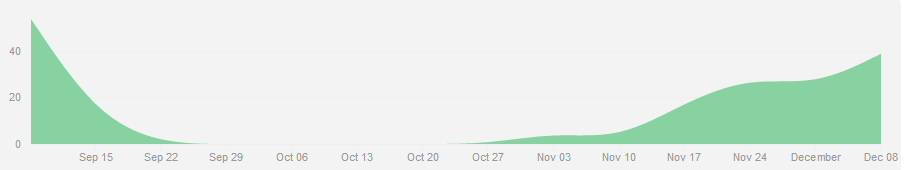
\includegraphics[scale = 0.5]{Billeder/Githubcommits.png}
\caption{Antal commits over projektets forl�b}
\label{fig:Githubcommits}
\end{figure}

\subfile{5_1_Sprint1}
\subfile{5_2_Sprint2}
\subfile{5_3_Sprint3}
\subfile{5_4_Sprint4}
\subfile{5_5_Sprint5}
\subfile{5_6_Sprint6}
\subfile{5_7_Sprint7}
\subfile{5_8_Sprint8}
\subfile{5_9_Sprint9}


\end{document}